\section{Where We Left Off}


\begin{frame}{A Recurring Issue}
    \begin{itemize}
        \item Lecture 4: $\Var(\hat\beta_j)=\sigma^2[(\bX'\bX)^{-1}]_{jj}$, which becomes large when $\bx_j$ is close to a linear combination of the other regressors.
        \item Lecture 8: centering $x_1$ and $x_2$ reduced the correlation between $x_1x_2$ and its components.
        \item Lecture 9, gasoline mileage: all five $t$-tests insignificant ($p>0.2$), yet the overall $F_0=14.66$ ($p\approx10^{-6}$). Horsepower and torque are correlated at $0.96$.
        \item Lecture 9, delivery time: adjusting distance for cases left only $1-0.824^2=0.321$ of its variation, and $1/0.321=3.12$ was called the variance inflation factor.
    \end{itemize}
    \svspace{0.5em}
    This lecture gives the problem a name, measures it, and looks at what can be done about it.
\end{frame}


\begin{frame}{Datasets in This Lecture}
    \begin{center}
        \footnotesize
        \begin{tabular}{llc}
            \toprule
            Data & MPV & $n$ \\
            \midrule
            Acetylene & Table 9.1 & 16 \\
            Webster, Gunst \& Mason & Table 9.4 & 12 \\
            Gasoline mileage & Table B.3 & 30 \\
            Hald cement & Table B.21 & 13 \\
            Delivery time & Example 3.1 & 25 \\
            Windmill & Table 5.5 & 25 \\
            % Simulated & --- & 30 \\
            \bottomrule
        \end{tabular}
    \end{center}
    MPV = Montgomery, Peck \& Vining, \emph{Introduction to Linear Regression Analysis}, 5th ed.
\end{frame}


\begin{frame}{The Datasets, Briefly}
    \footnotesize
    \begin{itemize}
        \item \textbf{Acetylene}: percentage conversion of $n$-heptane to acetylene in 16 runs of a chemical process; $x_1$ = reactor temperature ($^\circ$C), $x_2$ = ratio of H$_2$ to $n$-heptane (mole ratio), $x_3$ = contact time (s).
        \item \textbf{Webster, Gunst \& Mason}: 12 observations on $y$ and six regressors; $x_1+x_2+x_3+x_4$ is close to 10 in every row.
        \item \textbf{Gasoline mileage}: miles per gallon of 32 automobiles (30 with complete data) and ten design variables: displacement, horsepower, torque, compression ratio, rear axle ratio, carburetor barrels, transmission speeds, length, width, weight.
        \item \textbf{Hald cement}: heat evolved (cal/g) by 13 cement samples during hardening; $x_1$--$x_4$ are the percentages of four compounds in the clinker.
        \item \textbf{Delivery time}: vending-machine delivery time against cases stocked and distance walked.
        \item \textbf{Windmill}: DC output of a windmill against wind velocity.
    \end{itemize}
\end{frame}


\begin{frame}{Data Sources}
    \footnotesize
    \begin{itemize}
        \setlength{\itemsep}{0.2em}
        \item Acetylene: Kunugi, T., Tamura, T.\ and Naito, T.\ (1961), \emph{Chemical Engineering Progress} 57(11); analysed by Marquardt, D.\ W.\ and Snee, R.\ D.\ (1975), Ridge regression in practice, \emph{The American Statistician} 29(1), 3--20.
        \item Webster, J.\ T., Gunst, R.\ F.\ and Mason, R.\ L.\ (1974), Latent root regression analysis, \emph{Technometrics} 16(4), 513--522.
        \item Gasoline mileage: \emph{Motor Trend} (1975), as reproduced in MPV Table B.3.
        \item Hald cement: Woods, H., Steinour, H.\ H.\ and Starke, H.\ R.\ (1932), Effect of composition of Portland cement on heat evolved during hardening, \emph{Industrial and Engineering Chemistry} 24(11), 1207--1214; Hald, A.\ (1952), \emph{Statistical Theory with Engineering Applications}.
        \item Windmill: Joglekar, G., Schuenemeyer, J.\ H.\ and LaRiccia, V.\ (1989), Lack-of-fit testing when replicates are not available, \emph{The American Statistician} 43(3), 135--143.
        \item Delivery time: MPV Example 3.1.
    \end{itemize}
\end{frame}


\section{What Multicollinearity Is}


\begin{frame}{Linear Dependence Among the Regressors}
    Write the regressor columns (without the intercept) as $\bx_1,\dots,\bx_k$.
    \svspace{0.5em}
    \begin{itemize}
        \item \textbf{Exact dependence}: constants $t_1,\dots,t_k$, not all zero, with
        \[
        \sum_{j=1}^k t_j(\bx_j-\bar x_j\bone)=\bzero.
        \]
        Then $\bX'\bX$ is singular and $\bbeta$ has no unique least-squares estimate.
        \item \textbf{Near dependence}: the same combination is close to $\bzero$. $\bX'\bX$ is invertible but nearly singular.
        \item \textbf{Multicollinearity} means a near dependence among the regressors. Exact dependence is rare in practice and is usually a coding error (for example, a dummy for every level of a factor).
    \end{itemize}
\end{frame}


\begin{frame}{Unit-Length Scaling}
    To compare regressors measured in different units, center and scale each column:
    \[
    w_{ij}=\frac{x_{ij}-\bar x_j}{\sqrt{S_{jj}}},\qquad S_{jj}=\sum_{i=1}^n(x_{ij}-\bar x_j)^2 .
    \]
    \begin{itemize}
        \item Each column $\bw_j$ has mean $0$ and length $1$: $\bw_j'\bw_j=1$.
        \item $\bw_j'\bw_l=r_{jl}$, the correlation between regressors $x_j$ and $x_l$, so $\bW'\bW$ is the \textbf{correlation matrix} of the regressors.
        \item Scaling $y$ the same way gives the model $\by^*=\bW\bb+\bvarepsilon^*$ with no intercept. The fitted coefficients $\hat b_j=\hat\beta_j\sqrt{S_{jj}/\SST}$ are unit-free.
        \item The errors are scaled too: $\bvarepsilon^*=\bvarepsilon/\sqrt{\SST}$ has variance $\sigma_w^2=\sigma^2/\SST$.
    \end{itemize}
    All diagnostics in this lecture use $\bW'\bW$, so they do not depend on the units of the regressors.
\end{frame}


\begin{frame}{Sources of Multicollinearity}
    \begin{enumerate}
        \item \textbf{Data collection}: only a subspace of the regressor space was sampled. Acetylene: temperature and contact time were changed together.
        \item \textbf{Constraints in the model or population}: Hald cement, where the four compound percentages add up to 95--99; Webster data, where $x_1+x_2+x_3+x_4\approx10$.
        \item \textbf{Model specification}: polynomial or interaction terms. Windmill: over the observed range of wind velocity, $x$ and $x^2$ are almost collinear.
        \item \textbf{Overdefined model}: more regressors than observations, or nearly so, as in some medical and genetic studies.
    \end{enumerate}
    The first source can be fixed by collecting more data. The second cannot: the constraint is a property of the population.
\end{frame}


\begin{frame}{Acetylene Data: How the Data Were Collected}
    \begin{columns}[T]
        \begin{column}{0.5\textwidth}
            \begin{itemize}
                \item 16 runs at three temperatures: 1100, 1200 and 1300$^\circ$C.
                \item Contact time is long at low temperature and short at high temperature.
                \item $r(x_1,x_3)=-0.958$.
                \item No runs at high temperature with long contact time, or at low temperature with short contact time.
            \end{itemize}
        \end{column}
        \begin{column}{0.5\textwidth}
            \centering
            % Figure: acetylene_x1_x3.pdf (see multicollinearity-acetylene.R)
            \mode<presentation>{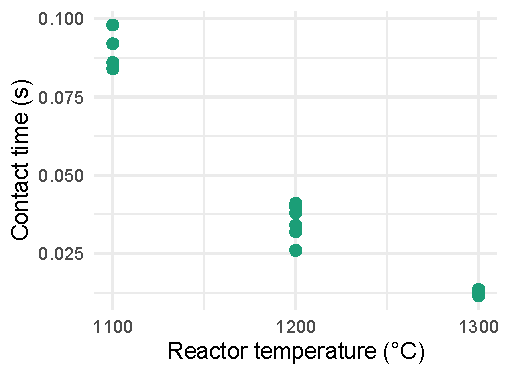
\includegraphics[width=\linewidth]{figures/acetylene_x1_x3.pdf}}
            \mode<article>{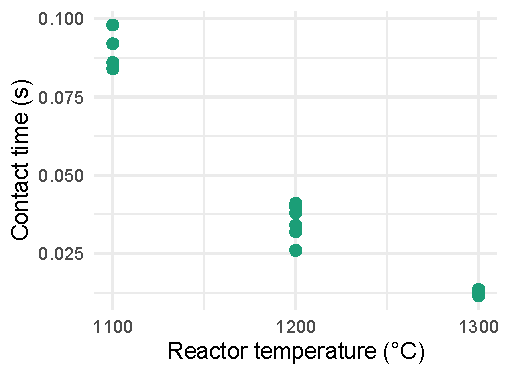
\includegraphics[width=0.8\linewidth]{figures/acetylene_x1_x3.pdf}}
        \end{column}
    \end{columns}
\end{frame}


\begin{frame}{Acetylene Data: The Model}
    MPV fits a full quadratic model in the three regressors, after scaling each to mean 0 and standard deviation 1:
    \[
    y=\beta_0+\sum_{j=1}^3\beta_jx_j+\beta_{12}x_1x_2+\beta_{13}x_1x_3+\beta_{23}x_2x_3+\sum_{j=1}^3\beta_{jj}x_j^2+\varepsilon
    \]
    \begin{itemize}
        \item $k=9$ regressors, $p=10$ parameters, $n=16$: only 6 residual degrees of freedom.
        \item Least squares: $R^2=0.9977$, $\MSRes=0.8126$.
        \item Since $x_1\approx-x_3$ in the scaled data, products of $x_1$ resemble products of $x_3$: $x_1x_3\approx-x_1^2$ and $x_1x_2\approx-x_2x_3$. The quadratic terms add new near dependencies.
    \end{itemize}
\end{frame}


\begin{frame}{Question: Is Multicollinearity a Property of the Model or of the Data?}
    \begin{itemize}
        \item The acetylene runs could, in principle, be repeated at other operating conditions. The cement percentages cannot be made to sum to anything other than about 100.
        \item In which case would more data remove the problem?
    \end{itemize}
    % Answer:
    % - Multicollinearity is a condition of the observed X matrix, not of the error distribution or of beta.
    % - For the acetylene data it comes from where the runs were made; new runs at high temperature with long contact time (if the process allows them) would break the dependency.
    % - For the cement data the dependency is built into the population: every sample's percentages sum to about 100, so more samples of the same kind cannot remove it.
\end{frame}


\section{Effects of Multicollinearity}


\begin{frame}{Two Regressors}
    In unit-length form with two regressors,
    \[
    \bW'\bW=\begin{bmatrix}1&r_{12}\\r_{12}&1\end{bmatrix},
    \qquad
    \bC=(\bW'\bW)^{-1}=\frac{1}{1-r_{12}^2}\begin{bmatrix}1&-r_{12}\\-r_{12}&1\end{bmatrix}.
    \]
    \begin{itemize}
        \item $\Var(\hat b_1)=\Var(\hat b_2)=\sigma_w^2/(1-r_{12}^2)$.
        \item $\Cov(\hat b_1,\hat b_2)=-r_{12}\,\sigma_w^2/(1-r_{12}^2)$, so $\Corr(\hat b_1,\hat b_2)=-r_{12}$.
        \item As $|r_{12}|\to1$ both variances grow without bound, and the estimates become strongly correlated, with the opposite sign to $r_{12}$.
    \end{itemize}
    \svspace{0.5em}
    From here on $\bC$ means $(\bW'\bW)^{-1}$, not Lecture 4's $(\bX'\bX)^{-1}$. For a slope coefficient the two are related by $[(\bX'\bX)^{-1}]_{jj}=C_{jj}/S_{jj}$.
\end{frame}


\begin{frame}{Simulation: Sampling Distribution of $(\hat\beta_1,\hat\beta_2)$}
    $y=1+2x_1+2x_2+\varepsilon$, $\sigma=1$, $n=30$, the same $\bX$ in 2000 replicates; $x_1,x_2$ have sample standard deviation 1.
    \begin{center}
        % Figure: sim_beta_scatter.pdf (see multicollinearity-simulation.R)
        \mode<presentation>{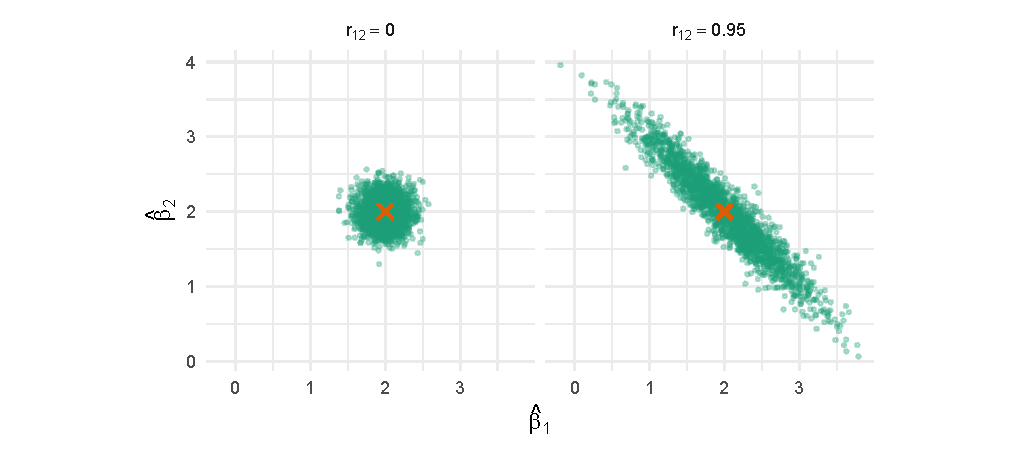
\includegraphics[width=0.75\linewidth]{figures/sim_beta_scatter.pdf}}
        \mode<article>{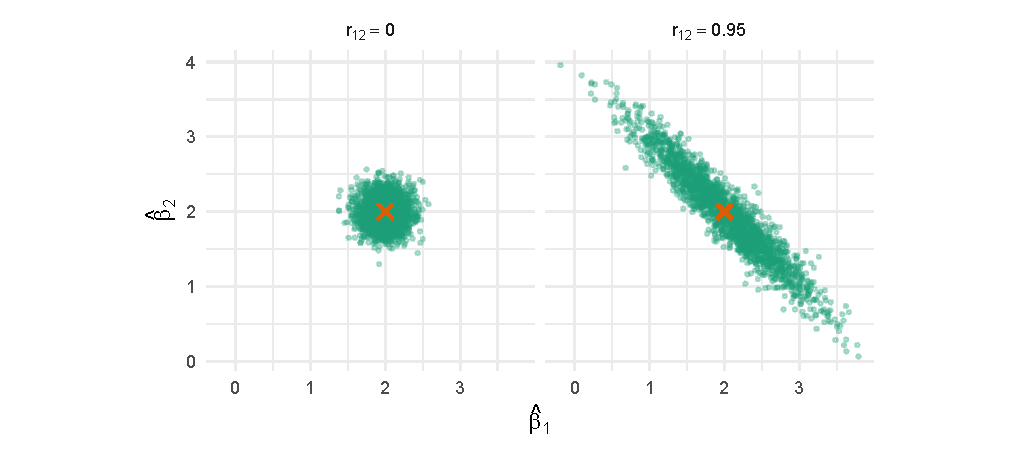
\includegraphics[width=0.9\linewidth]{figures/sim_beta_scatter.pdf}}
    \end{center}
    \vspace{-0.5em}
    $r_{12}=0$: $\operatorname{sd}(\hat\beta_1)=0.18$. $r_{12}=0.95$: $\operatorname{sd}(\hat\beta_1)=0.60$ (theory $0.595$) and $\Corr(\hat\beta_1,\hat\beta_2)=-0.95$.
\end{frame}


\begin{frame}{Some Combinations Are Still Well Estimated}
    With $\bC$ from the two-regressor case,
    \begin{align*}
        \Var(\hat b_1+\hat b_2) &= \sigma_w^2\,\frac{2-2r_{12}}{1-r_{12}^2}=\frac{2\sigma_w^2}{1+r_{12}}, \\
        \Var(\hat b_1-\hat b_2) &= \sigma_w^2\,\frac{2+2r_{12}}{1-r_{12}^2}=\frac{2\sigma_w^2}{1-r_{12}}.
    \end{align*}
    \begin{itemize}
        \item For $r_{12}=0.95$: the sum has variance $1.03\sigma_w^2$, the difference $40\sigma_w^2$.
        \item In the scatter plot, the cloud stretches along the line $\hat\beta_1+\hat\beta_2=4$ and is narrow across it.
        \item The data say a lot about the combined effect of $x_1$ and $x_2$, and little about how to split it between them.
    \end{itemize}
\end{frame}


\begin{frame}{The General Case}
    For $k$ regressors in unit-length form, $\bC=(\bW'\bW)^{-1}$ and
    \[
    C_{jj}=\frac{1}{1-R_j^2},
    \qquad
    \Var(\hat b_j)=\frac{\sigma_w^2}{1-R_j^2},
    \]
    where $R_j^2$ is the coefficient of determination from regressing $x_j$ on the other $k-1$ regressors (derived in the VIF section). Since $\hat\beta_j=\hat b_j\sqrt{\SST/S_{jj}}$ and $\sigma_w^2=\sigma^2/\SST$, in original units
    \[
    \Var(\hat\beta_j)=\frac{\sigma^2}{S_{jj}}\cdot\frac{1}{1-R_j^2},
    \]
    the same formula as in the added-variable plot of Lecture 9.
\end{frame}


\begin{frame}{The Estimates Are Too Long on Average}
    Let $L^2=(\hat{\bb}-\bb)'(\hat{\bb}-\bb)$ be the squared distance from the estimate to the true coefficients. With eigenvalues $\lambda_1,\dots,\lambda_k$ of $\bW'\bW$,
    \begin{align*}
        \E(L^2) &= \sum_{j=1}^k\Var(\hat b_j)=\sigma_w^2\tr(\bW'\bW)^{-1}=\sigma_w^2\sum_{j=1}^k\frac{1}{\lambda_j}, \\
        \E(\hat{\bb}'\hat{\bb}) &= \bb'\bb+\sigma_w^2\sum_{j=1}^k\frac{1}{\lambda_j}.
    \end{align*}
    \begin{itemize}
        \item The trace of a matrix is the sum of its eigenvalues, and the eigenvalues of $(\bW'\bW)^{-1}$ are $1/\lambda_j$.
        \item One small $\lambda_j$ is enough to make $\E(L^2)$ large. Orthogonal regressors have all $\lambda_j=1$ and $\E(L^2)=k\sigma_w^2$.
    \end{itemize}
\end{frame}


\begin{frame}{Acetylene Data: Length of the Estimate}
    \begin{itemize}
        \item $\sum_j1/\lambda_j=10{,}610$, against $9$ for orthogonal regressors.
        \item In the unit-length scale, $\hat\sigma_w^2=\MSRes/\SST=0.8126/2123.7=0.000383$.
        \item Least squares: $\hat{\bb}'\hat{\bb}=6.77$.
        \item Expected inflation from noise alone: $\hat\sigma_w^2\sum_j1/\lambda_j=0.000383\times10{,}610=4.06$.
    \end{itemize}
    \svspace{0.5em}
    More than half of the squared length of the least-squares coefficient vector can be accounted for by the variance, not by the true coefficients.
\end{frame}


\begin{frame}{Symptoms in a Fitted Model}
    \begin{itemize}
        \item Large standard errors and wide confidence intervals.
        \item Individual $t$-tests insignificant while the overall $F$-test is highly significant.
        \item Coefficients with the wrong sign or an implausible size.
        \item Estimates that change a lot when an observation or a regressor is added or removed.
    \end{itemize}
    \svspace{0.5em}
    Gasoline mileage, all ten regressors: $R^2=0.829$ and $F_0=9.18$ on $(10,19)$ df, yet no $t$-test is significant at 5\%. Displacement gets $-0.100$ but torque gets $+0.126$, although both are correlated about $-0.85$ with mileage.
\end{frame}


\begin{frame}{Prediction Is Not Always Hurt}
    \[
    \Var(\hat y_0)=\sigma^2\,\bx_0'(\bX'\bX)^{-1}\bx_0
    \]
    \begin{itemize}
        \item If $\bx_0$ follows the same pattern as the data (acetylene: high temperature with short contact time), $\hat y_0$ is precise: the errors in the correlated $\hat\beta_j$ cancel through their covariances (next slide).
        \item If $\bx_0$ breaks the pattern (high temperature with long contact time), the prediction depends on exactly those directions the data cannot estimate, and $\Var(\hat y_0)$ is large.
        \item Multicollinearity is mainly a problem for \emph{interpreting} coefficients and for \emph{extrapolating} outside the region of the data.
    \end{itemize}
\end{frame}


\begin{frame}{Why the Errors Cancel: Two Regressors}
    In unit-length form, a new point $(w_{01},w_{02})$ has
    \[
    \Var(w_{01}\hat b_1+w_{02}\hat b_2)=\sigma_w^2\,\frac{w_{01}^2+w_{02}^2-2r_{12}\,w_{01}w_{02}}{1-r_{12}^2}.
    \]
    \begin{center}
        \footnotesize
        \begin{tabular}{lcc}
            \toprule
            & $r_{12}>0$ & $r_{12}<0$ (acetylene) \\
            \midrule
            Data pattern & rise together & one up, one down \\
            $\Cov(\hat b_1,\hat b_2)$ & $<0$: errors opposite & $>0$: errors alike \\
            Point along the pattern & $w_{02}=w_{01}$ & $w_{02}=-w_{01}$ \\
            Weights on the errors & same sign & opposite signs \\
            Variance along the pattern (small) & $2w_{01}^2\sigma_w^2/(1+|r_{12}|)$ & $2w_{01}^2\sigma_w^2/(1+|r_{12}|)$ \\
            Variance against it (large) & $2w_{01}^2\sigma_w^2/(1-|r_{12}|)$ & $2w_{01}^2\sigma_w^2/(1-|r_{12}|)$ \\
            \bottomrule
        \end{tabular}
    \end{center}
    Whatever the sign of $r_{12}$, the errors cancel when the new point lies along the pattern of the data.
\end{frame}


\begin{frame}{Question: Does Multicollinearity Bias Least Squares?}
    \begin{itemize}
        \item The Gauss--Markov conditions still hold. Is $\hat{\bbeta}$ still unbiased? Still BLUE?
        \item If so, what exactly is the problem?
    \end{itemize}
    % Answer:
    % - Yes: E(beta_hat) = beta and it is still the minimum-variance linear unbiased estimator. Nothing in Lecture 4's proofs needed the columns to be uncorrelated.
    % - The problem is that the minimum variance among unbiased estimators is itself very large.
    % - This opens the door to biased estimators with much smaller variance (ridge, PCR), which can have smaller mean squared error.
\end{frame}


\section{Detection: The Correlation Matrix}


\begin{frame}{Inspecting $\bW'\bW$}
    The off-diagonal elements $r_{jl}$ of $\bW'\bW$ are the pairwise correlations between regressors.
    \begin{itemize}
        \item $|r_{jl}|$ close to 1 signals a near dependence between $x_j$ and $x_l$.
        \item Easy to compute and to read, and it shows \emph{which} pair is involved.
    \end{itemize}
    \svspace{0.5em}
    Acetylene, original regressors: $r(x_1,x_3)=-0.958$, $r(x_1,x_2)=0.224$, $r(x_2,x_3)=-0.240$.

    Among the nine terms of the quadratic model, the largest correlations are
    \begin{center}
        \footnotesize
        \begin{tabular}{lr@{\qquad}lr}
            \toprule
            Pair & $r$ & Pair & $r$ \\
            \midrule
            $x_1x_2$, $x_2x_3$ & $-0.974$ & $x_1$, $x_3$ & $-0.958$ \\
            $x_1x_3$, $x_1^2$ & $-0.972$ & $x_1^2$, $x_3^2$ & $0.894$ \\
            $x_1x_3$, $x_3^2$ & $-0.972$ & $x_3$, $x_3^2$ & $0.765$ \\
            \bottomrule
        \end{tabular}
    \end{center}
\end{frame}


\begin{frame}{Gasoline Mileage: Correlation Matrix}
    \begin{columns}[T]
        \begin{column}{0.42\textwidth}
            \footnotesize
            Six pairs exceed $0.9$:
            \begin{itemize}
                \item displacement--torque $0.990$
                \item horsepower--torque $0.964$
                \item displacement--horsepower $0.941$
                \item length--weight $0.934$
                \item displacement--weight $0.924$
                \item torque--weight $0.910$
            \end{itemize}
            Displacement, horsepower, torque and weight all measure the size of the car.
        \end{column}
        \begin{column}{0.58\textwidth}
            \centering
            % Figure: gas_corr_heatmap.pdf (see multicollinearity-gasoline.R)
            \mode<presentation>{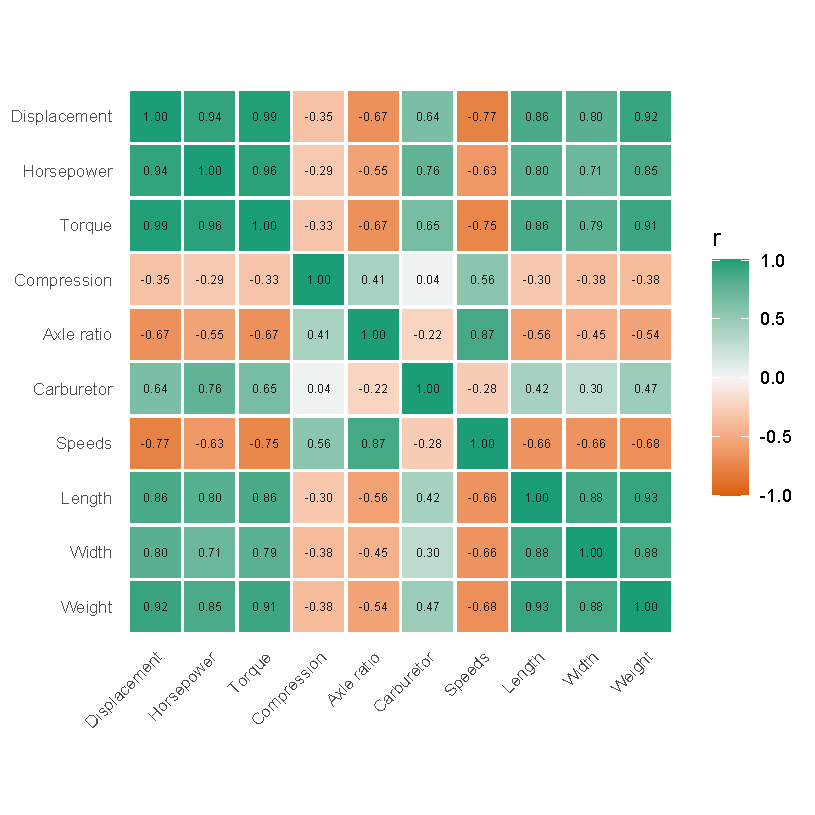
\includegraphics[height=0.78\textheight]{figures/gas_corr_heatmap.pdf}}
            \mode<article>{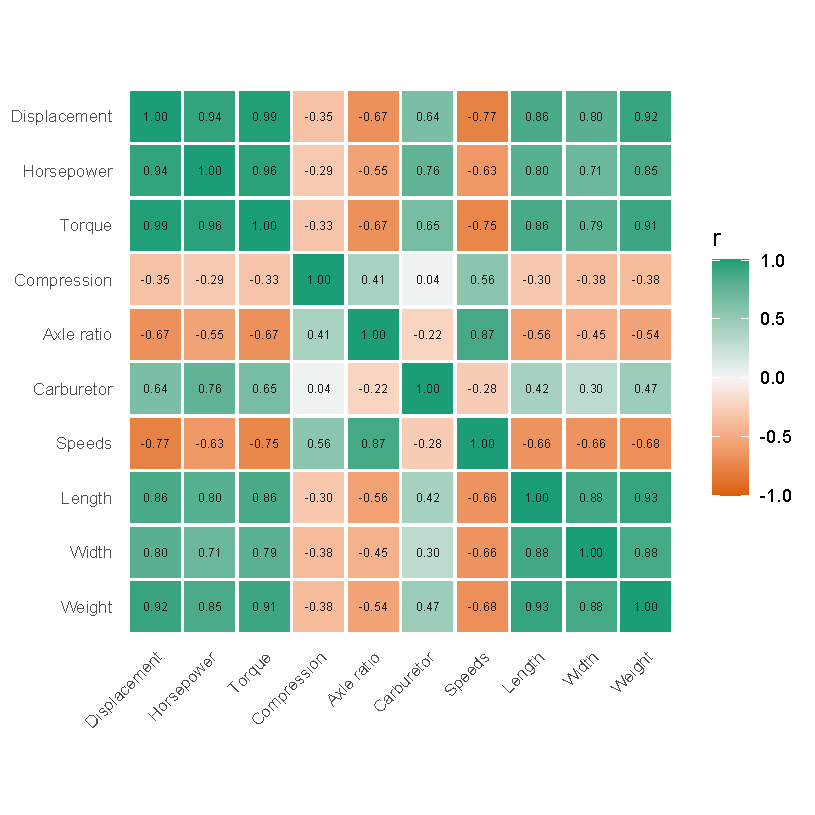
\includegraphics[width=0.8\linewidth]{figures/gas_corr_heatmap.pdf}}
        \end{column}
    \end{columns}
\end{frame}


\begin{frame}{Gasoline Mileage: The Four Size Variables}
    \begin{center}
        % Figure: gas_pairs.pdf (see multicollinearity-gasoline.R)
        \mode<presentation>{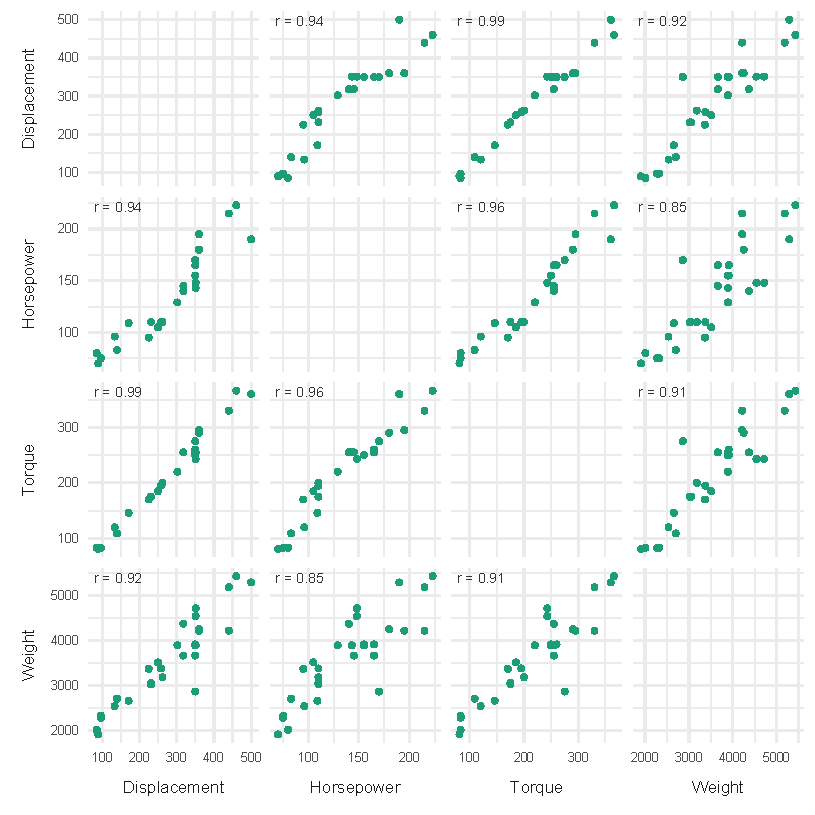
\includegraphics[height=0.78\textheight]{figures/gas_pairs.pdf}}
        \mode<article>{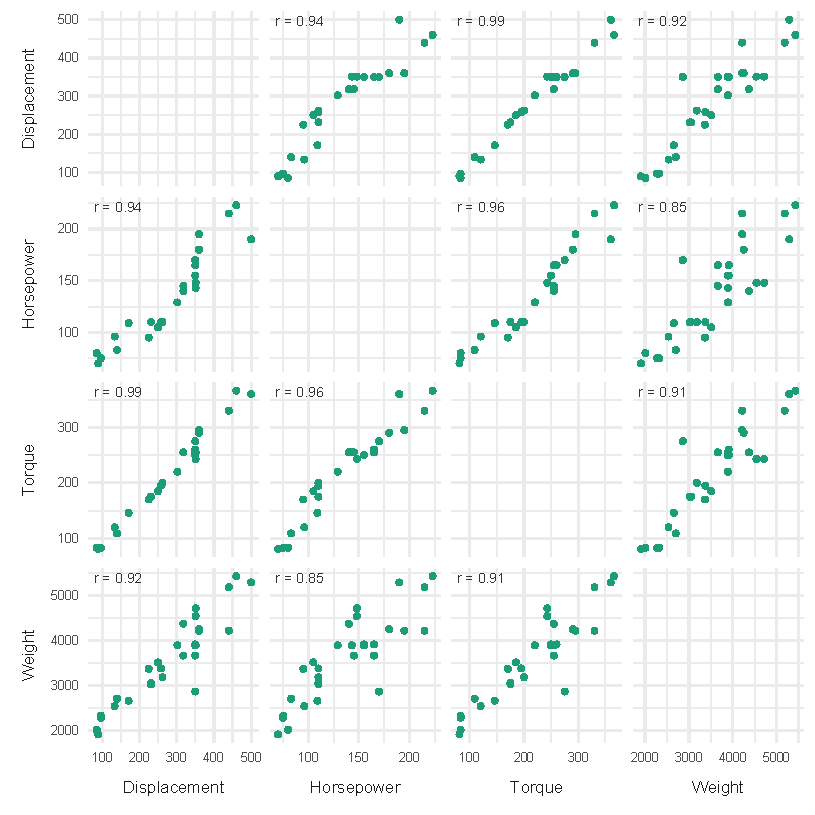
\includegraphics[width=0.7\linewidth]{figures/gas_pairs.pdf}}
    \end{center}
\end{frame}


\begin{frame}{Limitation: Only Pairs}
    A near dependence can involve three or more regressors without any large pairwise correlation.
    \svspace{0.5em}
    \begin{columns}[T]
        \begin{column}{0.45\textwidth}
            \footnotesize
            Webster, Gunst \& Mason data:
            \begin{itemize}
                \item Largest $|r_{jl}|$ is $0.505$.
                \item Yet $x_1+x_2+x_3+x_4=10$ in 11 of the 12 rows (11 in the first).
                \item The best single other regressor explains at most 26\% of the variation in any $x_j$.
                \item All the others together explain at least 99.4\% of each of $x_1,\dots,x_4$.
            \end{itemize}
        \end{column}
        \begin{column}{0.55\textwidth}
            \centering
            % Figure: webster_pairwise_vs_rj2.pdf (see multicollinearity-webster.R)
            \mode<presentation>{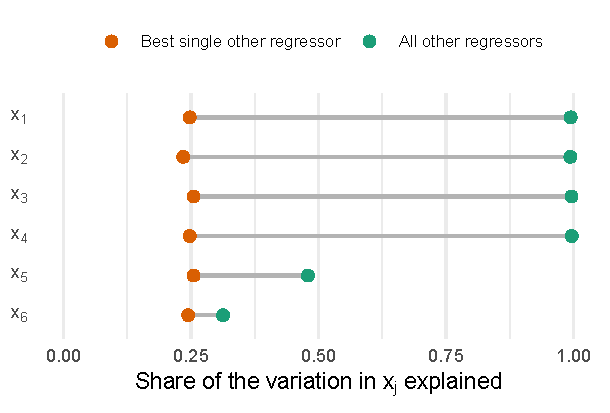
\includegraphics[width=\linewidth]{figures/webster_pairwise_vs_rj2.pdf}}
            \mode<article>{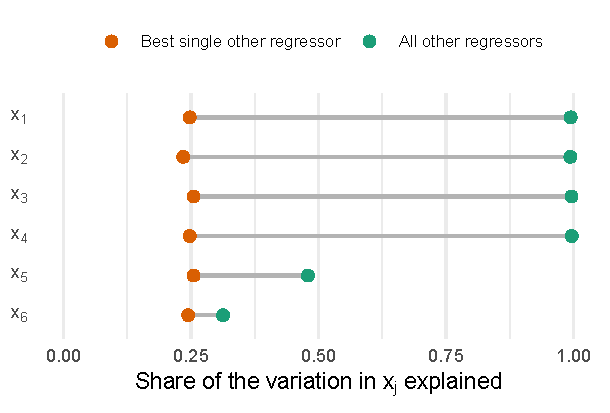
\includegraphics[width=0.8\linewidth]{figures/webster_pairwise_vs_rj2.pdf}}
        \end{column}
    \end{columns}
\end{frame}


\begin{frame}{Question: Is a Small Pairwise Correlation Reassuring?}
    \begin{itemize}
        \item With exactly two regressors, does a small $|r_{12}|$ rule out multicollinearity?
        \item With $k\ge3$ regressors, does it?
    \end{itemize}
    % Answer:
    % - With two regressors the only possible dependency is between x1 and x2, so |r12| tells the whole story: VIF = 1 / (1 - r12^2).
    % - With three or more, a combination such as x1 + x2 + x3 + x4 can be nearly constant while every pair is only moderately correlated (Webster data). The correlation matrix can miss it; VIF and eigenvalues will not.
\end{frame}


\section{Detection: Variance Inflation Factors}


\begin{frame}{Variance Inflation Factor}
    \[
    \VIF_j=C_{jj}=\bigl[(\bW'\bW)^{-1}\bigr]_{jj}=\frac{1}{1-R_j^2}
    \]
    \begin{itemize}
        \item $R_j^2$: coefficient of determination from regressing $x_j$ on the other regressors.
        \item $\Var(\hat\beta_j)=\dfrac{\sigma^2}{S_{jj}}\,\VIF_j$: the factor by which the variance is inflated compared with regressors that are uncorrelated with $x_j$.
        \item Standard errors and confidence intervals are inflated by $\sqrt{\VIF_j}$.
        \item $\VIF_j\ge1$, with equality when $x_j$ is uncorrelated with every other regressor.
    \end{itemize}
\end{frame}


\begin{frame}{Why $C_{jj}=1/(1-R_j^2)$}
    Put $\bw_j$ first: $\bW=[\bw_j\ \ \bW_{(-j)}]$. By the formula for the inverse of a partitioned matrix,
    \[
    C_{jj}=\Bigl[\bw_j'\bw_j-\bw_j'\bW_{(-j)}\bigl(\bW_{(-j)}'\bW_{(-j)}\bigr)^{-1}\bW_{(-j)}'\bw_j\Bigr]^{-1}
    =\Bigl[\bw_j'(\bI-\bH_{(-j)})\bw_j\Bigr]^{-1}.
    \]
    \begin{itemize}
        \item $\bw_j'(\bI-\bH_{(-j)})\bw_j$ is the residual sum of squares from regressing $\bw_j$ on $\bW_{(-j)}$.
        \item $\bw_j$ has mean 0 and $\bw_j'\bw_j=1$, so its total sum of squares is 1 and this residual sum of squares equals $1-R_j^2$.
        \item The same quantity appeared in Lecture 9 as the horizontal spread of the added-variable plot.
    \end{itemize}
\end{frame}


\begin{frame}{How Large Is Too Large?}
    \begin{columns}[T]
        \begin{column}{0.5\textwidth}
            \begin{itemize}
                \item Common guideline: $\VIF_j>5$ or $\VIF_j>10$ indicates a poorly estimated coefficient.
                \item $\VIF=10$ means $R_j^2=0.9$ and standard errors $\sqrt{10}=3.2$ times larger.
                \item With two regressors, $\VIF=1/(1-r_{12}^2)$; the delivery data ($r=0.824$) sit at $3.12$.
            \end{itemize}
        \end{column}
        \begin{column}{0.5\textwidth}
            \centering
            % Figure: sim_vif_curve.pdf (see multicollinearity-simulation.R)
            \mode<presentation>{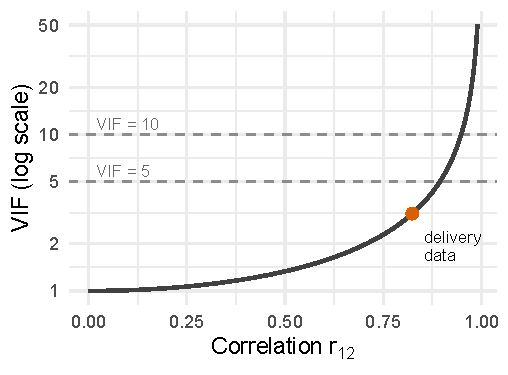
\includegraphics[width=\linewidth]{figures/sim_vif_curve.pdf}}
            \mode<article>{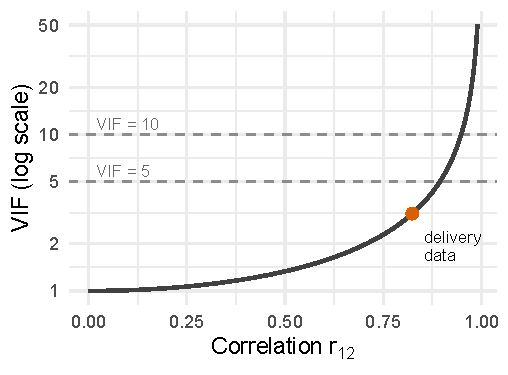
\includegraphics[width=0.8\linewidth]{figures/sim_vif_curve.pdf}}
        \end{column}
    \end{columns}
\end{frame}


\begin{frame}{Acetylene Data: VIFs}
    \begin{center}
        \small
        \begin{tabular}{lrr@{\qquad}lrr}
            \toprule
            Term & VIF & $R_j^2$ & Term & VIF & $R_j^2$ \\
            \midrule
            $x_1$ & 375.25 & 0.9973 & $x_2x_3$ & 35.61 & 0.9719 \\
            $x_2$ & 1.74 & 0.4255 & $x_1^2$ & 1762.58 & 0.9994 \\
            $x_3$ & 680.28 & 0.9985 & $x_2^2$ & 3.16 & 0.6840 \\
            $x_1x_2$ & 31.04 & 0.9678 & $x_3^2$ & 1156.77 & 0.9991 \\
            $x_1x_3$ & 6563.35 & 0.9998 & & & \\
            \bottomrule
        \end{tabular}
    \end{center}
    \begin{itemize}
        \item Every term involving temperature or contact time has a VIF above 30; the hydrogen ratio terms $x_2$ and $x_2^2$ are fine.
        \item The standard error of $\hat\beta_{13}$ is $\sqrt{6563}=81$ times what it would be with orthogonal regressors.
    \end{itemize}
\end{frame}


\begin{frame}{Gasoline Mileage: VIFs for All Ten Regressors}
    \begin{columns}[T]
        \begin{column}{0.45\textwidth}
            \begin{itemize}
                \item Five VIFs exceed 10: torque, displacement, horsepower, weight, length.
                \item Torque: $R_j^2=0.994$. The other nine regressors predict torque almost perfectly.
                \item Compression ratio is nearly unaffected.
            \end{itemize}
        \end{column}
        \begin{column}{0.55\textwidth}
            \centering
            % Figure: gas_vif_bar.pdf (see multicollinearity-gasoline.R)
            \mode<presentation>{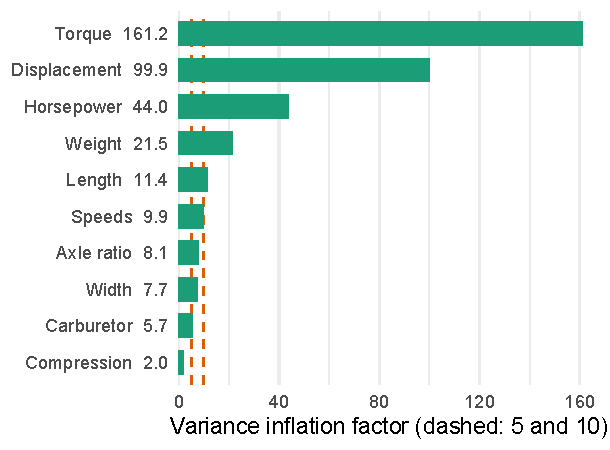
\includegraphics[width=\linewidth]{figures/gas_vif_bar.pdf}}
            \mode<article>{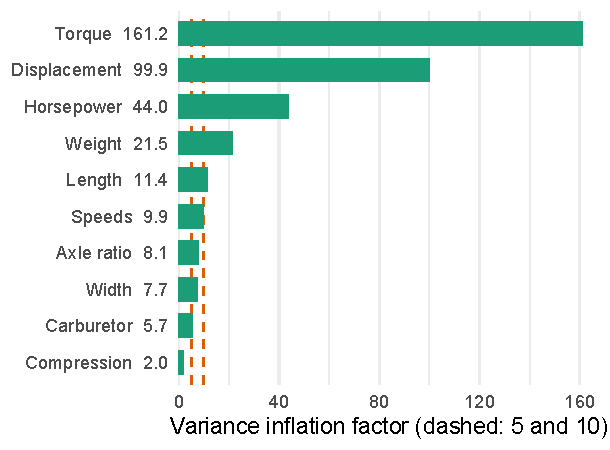
\includegraphics[width=0.8\linewidth]{figures/gas_vif_bar.pdf}}
        \end{column}
    \end{columns}
\end{frame}


\begin{frame}{Back to the Lecture 9 Puzzle}
    The five-regressor gasoline model: every $t$-test insignificant, $F_0=14.66$.
    \begin{center}
        \footnotesize
        \begin{tabular}{lrrr}
            \toprule
            Regressor & VIF & $\sqrt{\VIF}$ & $p$-value \\
            \midrule
            Horsepower & 29.05 & 5.4 & 0.882 \\
            Torque & 47.34 & 6.9 & 0.676 \\
            Rear axle ratio & 3.18 & 1.8 & 0.332 \\
            Carburetor barrels & 3.80 & 1.9 & 0.971 \\
            Weight & 8.98 & 3.0 & 0.205 \\
            \bottomrule
        \end{tabular}
    \end{center}
    \begin{itemize}
        \item The standard errors of horsepower and torque are five to seven times what they would be without collinearity.
        \item Each $t$-test asks whether $x_j$ helps \emph{given the others}. When the others carry the same information, the answer is no, even though the group as a whole matters.
    \end{itemize}
\end{frame}


\begin{frame}{Webster and Cement Data: VIFs}
    \begin{center}
        \small
        \begin{tabular}{lrrrrrr}
            \toprule
            & $x_1$ & $x_2$ & $x_3$ & $x_4$ & $x_5$ & $x_6$ \\
            \midrule
            Webster & 182.05 & 161.36 & 266.26 & 297.71 & 1.92 & 1.46 \\
            Hald cement & 38.50 & 254.42 & 46.87 & 282.51 & & \\
            \bottomrule
        \end{tabular}
    \end{center}
    \begin{itemize}
        \item Webster: the VIFs flag $x_1$--$x_4$ even though no pairwise correlation exceeds $0.51$.
        \item Cement: $R^2=0.982$ and the overall $F$-test is highly significant, yet no coefficient is significant at 5\%.
    \end{itemize}
\end{frame}


\begin{frame}{VIFs in R, and What They Do Not Tell}
    \begin{itemize}
        \item \texttt{car::vif(fit)}, or directly \texttt{diag(solve(cor(X)))} for a numeric regressor matrix \texttt{X}.
        \item VIFs say \emph{which} coefficients are poorly estimated.
        \item They do not say how many near dependencies there are, or which regressors take part in each. Acetylene: seven terms have VIF above 30. Is that one dependency or several?
    \end{itemize}
    \svspace{0.5em}
    The eigenvalues and eigenvectors of $\bW'\bW$ answer these questions.
\end{frame}


\begin{frame}{Question: Can a VIF Be Less Than 1?}
    \begin{itemize}
        \item Could adding a regressor correlated with $x_j$ ever make $\hat\beta_j$ \emph{more} precise?
    \end{itemize}
    % Answer:
    % - No: VIF_j = 1 / (1 - R_j^2) and 0 <= R_j^2 < 1, so VIF_j >= 1. Adding regressors can only increase R_j^2.
    % - In terms of sigma^2: adding a useful regressor can lower MSRes, which may shrink the estimated standard error overall even though the VIF goes up. The VIF isolates the effect of the design, holding sigma^2 fixed.
\end{frame}


\section{Detection: Eigensystem Analysis}


\begin{frame}{Eigenvalues of $\bW'\bW$}
    \[
    \bW'\bW=\bV\bLambda\bV',\qquad \bLambda=\operatorname{diag}(\lambda_1,\dots,\lambda_k),\quad\lambda_1\ge\cdots\ge\lambda_k>0
    \]
    \begin{itemize}
        \item $\bV=[\bv_1,\dots,\bv_k]$ is orthogonal: the eigenvectors are orthonormal.
        \item $\sum_j\lambda_j=\tr(\bW'\bW)=k$, since each diagonal element is 1.
        \item Orthogonal regressors: all $\lambda_j=1$.
        \item A near dependence shows up as a small eigenvalue:
        \[
        (\bW\bv_j)'(\bW\bv_j)=\bv_j'\bW'\bW\bv_j=\lambda_j .
        \]
        If $\lambda_j\approx0$, the combination $\bW\bv_j=\sum_l v_{lj}\bw_l$ is close to $\bzero$ for every observation.
    \end{itemize}
\end{frame}


\begin{frame}{Condition Number and Condition Indices}
    \[
    \kappa=\frac{\lambda_{\max}}{\lambda_{\min}},
    \qquad
    \kappa_j=\frac{\lambda_{\max}}{\lambda_j},\ j=1,\dots,k
    \]
    \begin{center}
        \small
        \begin{tabular}{ll}
            \toprule
            Condition number & Multicollinearity \\
            \midrule
            $\kappa<100$ & no serious problem \\
            $100\le\kappa\le1000$ & moderate to strong \\
            $\kappa>1000$ & severe \\
            \bottomrule
        \end{tabular}
    \end{center}
    \begin{itemize}
        \item The number of condition indices $\kappa_j$ above 1000 counts the near dependencies that are severe.
        \item $\det(\bW'\bW)=\prod_j\lambda_j$ lies between 0 and 1 and is close to 0 under multicollinearity, but it does not say how many dependencies there are.
    \end{itemize}
\end{frame}


\begin{frame}{Acetylene Data: Eigenvalues}
    \begin{center}
        \small
        \begin{tabular}{crr@{\qquad}crr}
            \toprule
            $j$ & $\lambda_j$ & $\kappa_j$ & $j$ & $\lambda_j$ & $\kappa_j$ \\
            \midrule
            1 & 4.2052 & 1.0 & 6 & 0.0495 & 84.9 \\
            2 & 2.1620 & 1.9 & 7 & 0.0136 & 308.6 \\
            3 & 1.1387 & 3.7 & 8 & 0.0051 & 820.1 \\
            4 & 1.0405 & 4.0 & 9 & 0.000097 & 43{,}381 \\
            5 & 0.3852 & 10.9 & & & \\
            \bottomrule
        \end{tabular}
    \end{center}
    \begin{itemize}
        \item $\kappa=43{,}381$: severe. One condition index exceeds 1000, two more lie between 100 and 1000.
        \item $\det(\bW'\bW)=1.4\times10^{-9}$.
        \item The eigenvalues sum to $9=k$, but four of them hold almost all of it.
    \end{itemize}
\end{frame}


\begin{frame}{Acetylene Data: Which Terms Are Involved?}
    Eigenvector for $\lambda_9=0.000097$:
    \begin{center}
        \small
        \begin{tabular}{ccccccccc}
            \toprule
            $x_1$ & $x_2$ & $x_3$ & $x_1x_2$ & $x_1x_3$ & $x_2x_3$ & $x_1^2$ & $x_2^2$ & $x_3^2$ \\
            \midrule
            0.174 & $-0.003$ & 0.237 & 0.003 & 0.797 & 0.008 & 0.412 & 0.005 & 0.329 \\
            \bottomrule
        \end{tabular}
    \end{center}
    \[
    0.17\,\bw_{x_1}+0.24\,\bw_{x_3}+0.80\,\bw_{x_1x_3}+0.41\,\bw_{x_1^2}+0.33\,\bw_{x_3^2}\approx\bzero
    \]
    \begin{itemize}
        \item Only temperature and contact time terms take part; the hydrogen ratio does not.
        \item The largest element of $\bW\bv_9$ is $0.0045$ in absolute value.
    \end{itemize}
\end{frame}


\begin{frame}{Webster Data: One Hidden Dependency}
    \begin{columns}[T]
        \begin{column}{0.5\textwidth}
            \small
            \begin{itemize}
                \item $\lambda$: 2.4288, 1.5462, 0.9221, 0.7940, 0.3079, 0.0011.
                \item $\kappa=2196$: severe, one near dependency.
                \item $\bv_6$ loads only on $x_1$--$x_4$.
                \item Dividing the loadings by the column lengths $\sqrt{S_{jj}}$ gives $1.00$, $1.06$, $1.05$, $1.05$, $0.04$, $0.03$: in original units the dependency is $x_1+x_2+x_3+x_4\approx$ constant.
            \end{itemize}
        \end{column}
        \begin{column}{0.5\textwidth}
            \centering
            % Figure: webster_eigvec.pdf (see multicollinearity-webster.R)
            \mode<presentation>{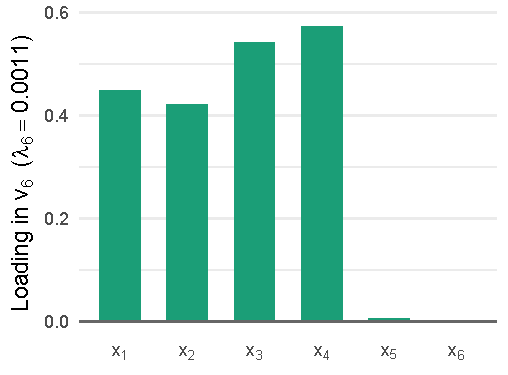
\includegraphics[width=\linewidth]{figures/webster_eigvec.pdf}}
            \mode<article>{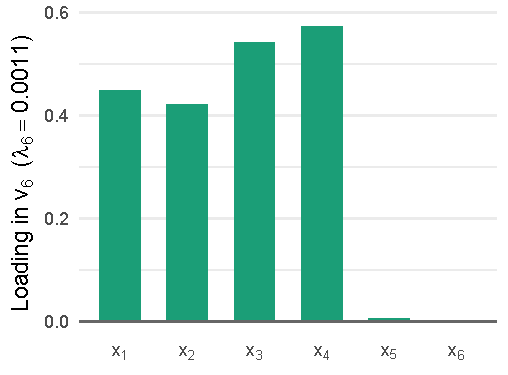
\includegraphics[width=0.8\linewidth]{figures/webster_eigvec.pdf}}
        \end{column}
    \end{columns}
\end{frame}


\begin{frame}{Gasoline Mileage: Condition Indices}
    \begin{columns}[T]
        \begin{column}{0.48\textwidth}
            \small
            \begin{itemize}
                \item $\kappa=1820$: severe.
                \item One $\kappa_j$ above 1000, two between 100 and 1000.
                \item Eigenvector of the smallest eigenvalue: displacement $0.55$, horsepower $0.31$, torque $-0.77$; all others below $0.08$ in absolute value.
                \item The worst dependency links displacement, horsepower and torque.
            \end{itemize}
        \end{column}
        \begin{column}{0.52\textwidth}
            \centering
            % Figure: gas_condition_indices.pdf (see multicollinearity-gasoline.R)
            \mode<presentation>{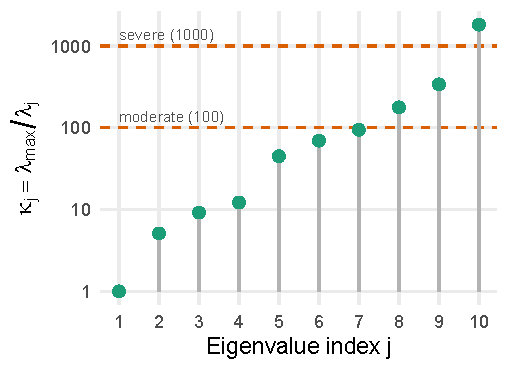
\includegraphics[width=\linewidth]{figures/gas_condition_indices.pdf}}
            \mode<article>{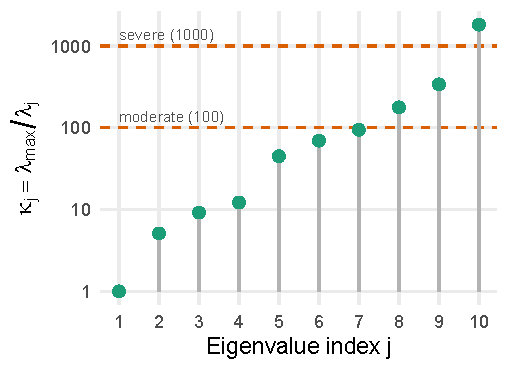
\includegraphics[width=0.8\linewidth]{figures/gas_condition_indices.pdf}}
        \end{column}
    \end{columns}
\end{frame}


\begin{frame}{Variance-Decomposition Proportions}
    Belsley, Kuh and Welsch (1980) split each variance by eigenvalue. From $\bC=\bV\bLambda^{-1}\bV'$,
    \[
    \VIF_j=C_{jj}=\sum_{s=1}^k\frac{v_{js}^2}{\lambda_s},
    \qquad
    \pi_{sj}=\frac{v_{js}^2/\lambda_s}{\VIF_j}.
    \]
    \begin{itemize}
        \item $\pi_{sj}$ is the share of $\Var(\hat b_j)$ that comes from eigenvalue $s$; each column of proportions sums to 1.
        \item Condition index $\eta_s=\sqrt{\lambda_{\max}/\lambda_s}$ (the square root of $\kappa_s$).
        \item Rule: a row with $\eta_s>30$ and two or more $\pi_{sj}>0.5$ marks a dependency among those regressors.
        \item Belsley, Kuh and Welsch use $\bX$ scaled to unit length but not centered, with the intercept column; here we use $\bW$ to match the rest of the lecture.
    \end{itemize}
\end{frame}


\begin{frame}{Acetylene Data: Variance-Decomposition Proportions}
    \begin{center}
        \small
        \begin{tabular}{rrccccccccc}
            \toprule
            $s$ & $\eta_s$ & $x_1$ & $x_2$ & $x_3$ & $x_1x_2$ & $x_1x_3$ & $x_2x_3$ & $x_1^2$ & $x_2^2$ & $x_3^2$ \\
            \midrule
            5 & 3.3 & .000 & .508 & .000 & .002 & .000 & .003 & .000 & .442 & .000 \\
            6 & 9.2 & .003 & .005 & .000 & .087 & .000 & .056 & .003 & .032 & .007 \\
            7 & 17.6 & .010 & .005 & .003 & \textbf{.822} & .000 & \textbf{.793} & .004 & .000 & .005 \\
            8 & 28.6 & .151 & .093 & .146 & .077 & .001 & .121 & .000 & .353 & .023 \\
            9 & 208.3 & \textbf{.835} & .065 & \textbf{.851} & .002 & \textbf{.999} & .020 & \textbf{.992} & .082 & \textbf{.965} \\
            \bottomrule
        \end{tabular}
    \end{center}
    Rows 1--4 are omitted (all proportions small except $x_2$: $0.290$ in row 4).
    \begin{itemize}
        \item Row 9: the temperature and contact time terms, as the eigenvector showed.
        \item Row 7 ($\eta=17.6$, below 30 but clear): $x_1x_2$ and $x_2x_3$, which are nearly opposite because $x_1\approx-x_3$.
    \end{itemize}
\end{frame}


\begin{frame}{Question: Why Must Some Eigenvalue Be Small?}
    \begin{itemize}
        \item The eigenvalues of $\bW'\bW$ always add up to $k$. If $\lambda_1=4.2$ for the acetylene data, what does that say about the others?
        \item Is a large $\lambda_1$ by itself a sign of multicollinearity?
    \end{itemize}
    % Answer:
    % - With sum fixed at k = 9 and lambda_1 = 4.2, the other eight share 4.8, so their average is 0.6 < 1.
    % - A large lambda_1 means the regressors share a common direction (they are correlated as a group); it forces some other eigenvalues below 1 but not necessarily close to 0.
    % - What matters for variances is how small the smallest eigenvalues are, since Var(b) involves 1/lambda_j; this is why kappa uses lambda_min.
\end{frame}


\section{Remedies}


\begin{frame}{Three Kinds of Remedy}
    \begin{enumerate}
        \item \textbf{Collect more data} so that the dependency is broken.
        \item \textbf{Respecify the model}: center, drop or combine regressors.
        \item \textbf{Use a biased estimator} with much smaller variance: ridge regression, principal-component regression.
    \end{enumerate}
    \svspace{0.5em}
    Which one fits depends on the source of the problem and on whether the goal is interpreting coefficients or predicting.
\end{frame}


\begin{frame}{Collecting Additional Data}
    \begin{itemize}
        \item New observations should fill the empty part of the regressor space. Acetylene: runs at high temperature with long contact time and at low temperature with short contact time.
        \item This is the best remedy when it is possible, because it removes the cause rather than working around it.
        \item Often it is not possible:
        \begin{itemize}
            \item the process may not run, or may be unsafe, at the missing combinations;
            \item observational data cannot be designed;
            \item a constraint in the population (cement percentages) holds in every new sample too.
        \end{itemize}
    \end{itemize}
\end{frame}


\begin{frame}{Respecification I: Centering Polynomial Terms}
    Windmill data, quadratic in wind velocity $x$ (range 2.45 to 10.2, mean 6.13):
    \begin{center}
        % Figure: windmill_centering.pdf (see multicollinearity-centering.R)
        \mode<presentation>{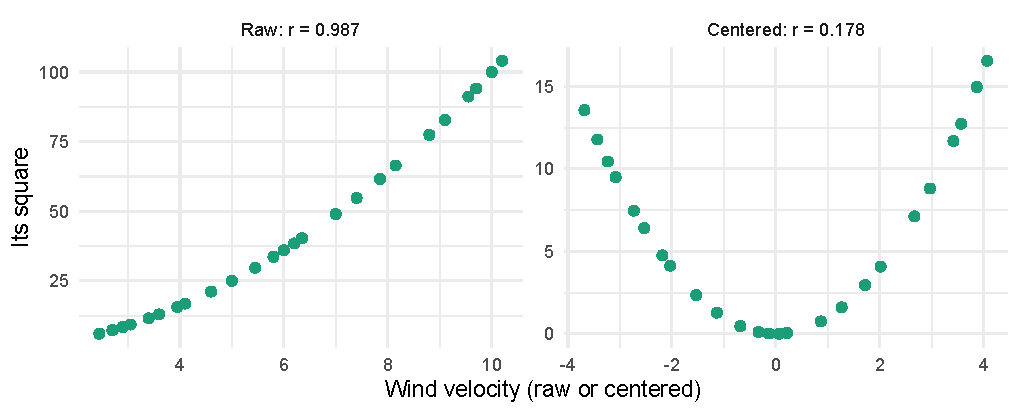
\includegraphics[width=0.8\linewidth]{figures/windmill_centering.pdf}}
        \mode<article>{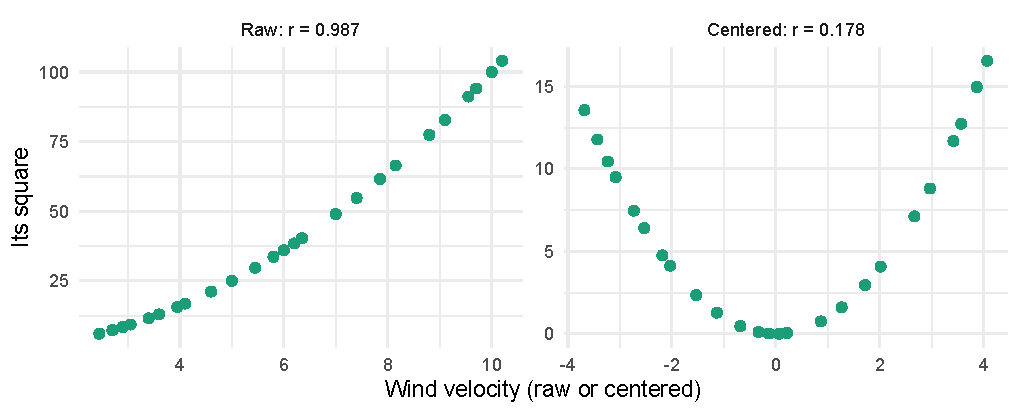
\includegraphics[width=0.9\linewidth]{figures/windmill_centering.pdf}}
    \end{center}
    \vspace{-0.5em}
    VIF falls from 38.5 to 1.03 when $x$ is replaced by $x-\bar x$.
\end{frame}


\begin{frame}{Centering Changes the Parameterization, Not the Fit}
    \begin{center}
        \small
        \begin{tabular}{lrr}
            \toprule
            & Raw $x$ & Centered $x-\bar x$ \\
            \midrule
            Intercept & $-1.156$ & $1.844$ \\
            Linear (se) & $0.7229\ (0.0614)$ & $0.2554\ (0.0101)$ \\
            Quadratic (se) & $-0.0381\ (0.0048)$ & $-0.0381\ (0.0048)$ \\
            \bottomrule
        \end{tabular}
    \end{center}
    \begin{itemize}
        \item Same fitted values, same $R^2$, same quadratic coefficient.
        \item The linear coefficient now means the slope at $x=\bar x$, which the data estimate well.
        \item Why it works: for $u=x-\bar x$, $\sum_iu_i\cdot u_i^2=\sum_iu_i^3$, which is close to 0 when the $u_i$ are spread symmetrically around 0. Far from 0, $x^2$ is almost a straight-line function of $x$.
        \item Centering does not help when the dependency is between different regressors: $\bW$ is already centered.
    \end{itemize}
\end{frame}


\begin{frame}{Respecification II: Dropping or Combining Regressors}
    Hald cement: drop $x_4$, which takes part in the near-sum constraint.
    \begin{center}
        \small
        \begin{tabular}{lrrr}
            \toprule
            & $x_1$ & $x_2$ & $x_3$ \\
            \midrule
            Estimate (se) & $1.696\ (0.205)$ & $0.657\ (0.044)$ & $0.250\ (0.185)$ \\
            VIF & 3.25 & 1.06 & 3.14 \\
            \bottomrule
        \end{tabular}
    \end{center}
    \begin{itemize}
        \item $R^2$ goes from $0.9824$ to $0.9823$: $x_4$ added almost nothing that $x_1$--$x_3$ did not already carry.
        \item Dropping a regressor whose true coefficient is not zero biases the others. Which regressors to keep is the subject of the next lecture.
        \item Combining: replace highly correlated regressors by one index (for example, a single measure of engine size in place of displacement, horsepower and torque).
    \end{itemize}
\end{frame}


\begin{frame}{Ridge Regression}
    In unit-length form, for a constant $\theta\ge0$,
    \[
    \hat{\bb}_R=(\bW'\bW+\theta\bI)^{-1}\bW'\by^*.
    \]
    \begin{itemize}
        \item $\theta=0$ gives least squares.
        \item Adding $\theta\bI$ adds $\theta$ to every eigenvalue: $\lambda_j\to\lambda_j+\theta$. The smallest eigenvalues, which caused the trouble, change the most in relative terms.
        \item Equivalently, $\hat{\bb}_R$ minimizes the penalized residual sum of squares
        \[
        (\by^*-\bW\bb)'(\by^*-\bW\bb)+\theta\,\bb'\bb .
        \]
        Setting the gradient $-2\bW'\by^*+2\bW'\bW\bb+2\theta\bb$ to zero gives $\hat{\bb}_R$. Large coefficients are penalized, so $\hat{\bb}_R$ is shorter than $\hat{\bb}$.
    \end{itemize}
\end{frame}


\begin{frame}{Ridge as Least Squares on Augmented Data}
    Append $k$ pseudo-observations: rows $\sqrt{\theta}\,\bI$ to $\bW$ and zeros to $\by^*$:
    \[
    \bW_A=\begin{bmatrix}\bW\\\sqrt{\theta}\,\bI\end{bmatrix},
    \qquad
    \by_A=\begin{bmatrix}\by^*\\\bzero\end{bmatrix}.
    \]
    \begin{itemize}
        \item $\bW_A'\bW_A=\bW'\bW+\theta\bI$ and $\bW_A'\by_A=\bW'\by^*$, so least squares on the augmented data gives $\hat{\bb}_R$.
        \item The pseudo-observations fill in the missing directions of the regressor space, with responses that pull the coefficients toward 0.
        \item Ridge regression can be fit with any least-squares routine.
    \end{itemize}
\end{frame}


\begin{frame}{Bias and Variance of the Ridge Estimator}
    $\hat{\bb}_R=\bZ_\theta\hat{\bb}$ with $\bZ_\theta=(\bW'\bW+\theta\bI)^{-1}\bW'\bW$, so
    \begin{align*}
        \E(\hat{\bb}_R) &= \bZ_\theta\bb\neq\bb\quad(\theta>0), \\
        \Var(\hat{\bb}_R) &= \sigma_w^2(\bW'\bW+\theta\bI)^{-1}\bW'\bW(\bW'\bW+\theta\bI)^{-1}.
    \end{align*}
    With $\balpha=\bV'\bb$ (coefficients along the eigenvectors), the mean squared error is
    \[
    \E\bigl[(\hat{\bb}_R-\bb)'(\hat{\bb}_R-\bb)\bigr]
    =\underbrace{\sigma_w^2\sum_{j=1}^k\frac{\lambda_j}{(\lambda_j+\theta)^2}}_{\text{total variance}}
    +\underbrace{\theta^2\sum_{j=1}^k\frac{\alpha_j^2}{(\lambda_j+\theta)^2}}_{\text{squared bias}}.
    \]
    \begin{itemize}
        \item The variance falls and the squared bias rises as $\theta$ increases.
        \item Hoerl and Kennard (1970): there is always some $\theta>0$ for which the ridge MSE is smaller than the least-squares MSE $\sigma_w^2\sum_j1/\lambda_j$.
    \end{itemize}
\end{frame}


\begin{frame}{Choosing $\theta$}
    \begin{itemize}
        \item \textbf{Ridge trace}: plot each $\hat b_{R,j}$ against $\theta$. Choose the smallest $\theta$ at which the coefficients have stabilized, have sensible signs, and $\SSRes$ has not grown much.
        \item \textbf{VIFs of the ridge estimator}: the diagonal of $(\bW'\bW+\theta\bI)^{-1}\bW'\bW(\bW'\bW+\theta\bI)^{-1}$; choose $\theta$ so that they are all small (they can fall below 1).
        \item \textbf{Hoerl, Kennard and Baldwin (1975)}: $\theta=k\hat\sigma_w^2/\hat{\bb}'\hat{\bb}$, with $\hat\sigma_w^2$ and $\hat{\bb}$ from least squares in the unit-length scale.
        \item \textbf{Cross-validation} or generalized cross-validation: choose $\theta$ to minimize prediction error.
    \end{itemize}
    \svspace{0.5em}
    The choice is a judgment call, and the methods often disagree.
\end{frame}


\begin{frame}{Acetylene Data: Ridge Trace}
    \begin{columns}[T]
        \begin{column}{0.4\textwidth}
            \small
            \begin{itemize}
                \item $x_1x_3$, $x_1^2$ and $x_3^2$ change most: the coefficient of $x_1x_3$ goes from $-2.03$ to $-0.19$ by $\theta=0.002$.
                \item The trace has flattened by $\theta\approx0.03$.
                \item We take $\theta=0.032$ (dashed line), the value MPV chooses.
                \item Square-root scale for $\theta$: most of the change happens at very small $\theta$.
            \end{itemize}
        \end{column}
        \begin{column}{0.6\textwidth}
            \centering
            % Figure: acetylene_ridge_trace.pdf (see multicollinearity-acetylene.R)
            \mode<presentation>{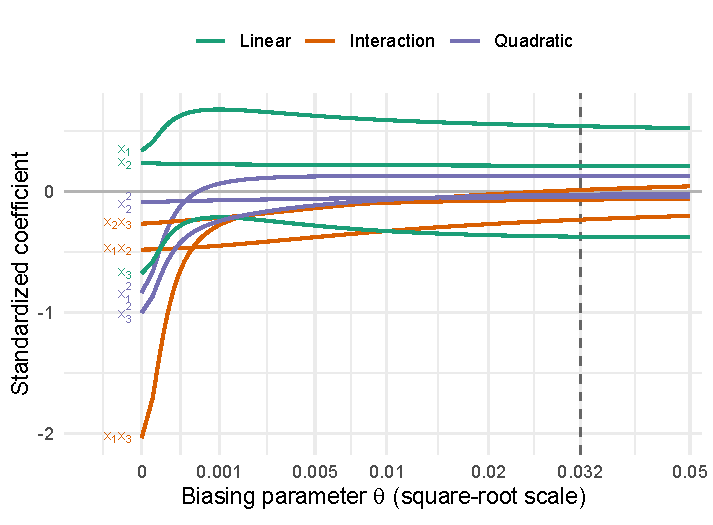
\includegraphics[width=\linewidth]{figures/acetylene_ridge_trace.pdf}}
            \mode<article>{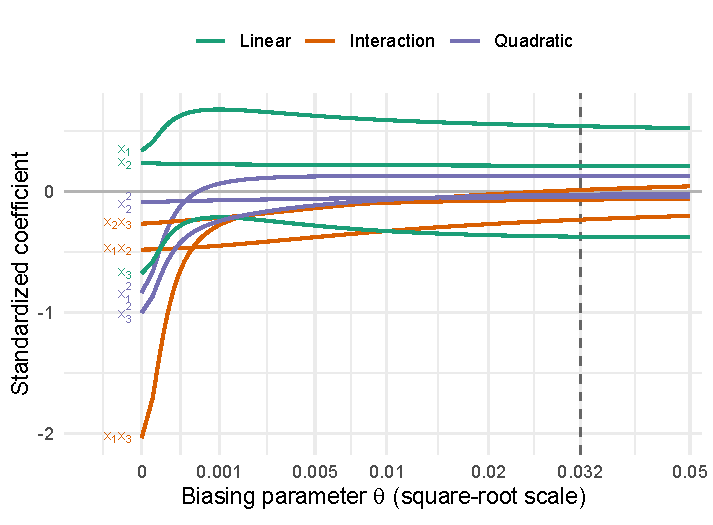
\includegraphics[width=0.8\linewidth]{figures/acetylene_ridge_trace.pdf}}
        \end{column}
    \end{columns}
\end{frame}


\begin{frame}{Acetylene Data: Fit and VIFs Along the Trace}
    \begin{center}
        \small
        \begin{tabular}{lrrrrrrr}
            \toprule
            $\theta$ & 0 & 0.001 & 0.005 & 0.01 & 0.02 & 0.032 & 0.05 \\
            \midrule
            $R^2$ & 0.9977 & 0.9972 & 0.9967 & 0.9961 & 0.9952 & 0.9944 & 0.9933 \\
            Largest VIF & 6563 & 76.0 & 27.0 & 12.4 & 6.39 & 4.18 & 2.63 \\
            \bottomrule
        \end{tabular}
    \end{center}
    \begin{itemize}
        \item A tiny $\theta$ removes most of the variance inflation at almost no cost in fit.
        \item At $\theta=0.032$: $\SSRes$ grows from $4.88$ to $11.92$, $R^2$ drops by $0.003$, and every VIF is below $4.2$.
        \item The Hoerl--Kennard--Baldwin rule gives $\theta=0.0005$, which leaves the largest VIF above 170. Here it shrinks far less than the trace suggests.
    \end{itemize}
\end{frame}


\begin{frame}{Acetylene Data: Least Squares vs.\ Ridge}
    Coefficients in the unit-length scale:
    \begin{center}
        \small
        \begin{tabular}{lrr@{\qquad}lrr}
            \toprule
            Term & LS & Ridge & Term & LS & Ridge \\
            \midrule
            $x_1$ & 0.337 & 0.539 & $x_2x_3$ & $-0.266$ & 0.012 \\
            $x_2$ & 0.234 & 0.212 & $x_1^2$ & $-0.835$ & 0.125 \\
            $x_3$ & $-0.676$ & $-0.374$ & $x_2^2$ & $-0.090$ & $-0.048$ \\
            $x_1x_2$ & $-0.480$ & $-0.233$ & $x_3^2$ & $-1.001$ & $-0.027$ \\
            $x_1x_3$ & $-2.034$ & $-0.068$ & & & \\
            \bottomrule
        \end{tabular}
    \end{center}
    \begin{itemize}
        \item $\hat{\bb}'\hat{\bb}$: $6.77$ for least squares, $0.55$ for ridge ($\theta=0.032$).
        \item The large least-squares coefficients of $x_1x_3$, $x_1^2$ and $x_3^2$ offset one another along the near dependency; ridge removes most of them.
    \end{itemize}
\end{frame}


\begin{frame}{Ridge Regression in R}
    \begin{itemize}
        \item By hand: \texttt{solve(crossprod(W) + theta * diag(ncol(W)), crossprod(W, ys))}, with \texttt{W} and \texttt{ys} scaled to unit length.
        \item \texttt{MASS::lm.ridge(y \textasciitilde{} ., data, lambda = n * theta)}: \texttt{lm.ridge} scales the regressors by their standard deviation with divisor $n$, so its \texttt{lambda} is $n$ times our $\theta$. \texttt{coef()} returns coefficients in the original units.
        \item \texttt{glmnet::glmnet(X, y, alpha = 0)} uses yet another scaling of the penalty, so its \texttt{lambda} is not comparable with $\theta$.
    \end{itemize}
    \svspace{0.5em}
    Always check which scaling a package uses before comparing values of $\theta$.
\end{frame}


\begin{frame}{Principal-Component Regression}
    Rotate the regressors onto the eigenvectors: $\bZ=\bW\bV$, $\balpha=\bV'\bb$.
    \[
    \by^*=\bW\bb+\bvarepsilon^*=\bZ\balpha+\bvarepsilon^*,
    \qquad
    \bZ'\bZ=\bV'\bW'\bW\bV=\bLambda.
    \]
    \begin{itemize}
        \item The columns of $\bZ$ (the principal components) are orthogonal, so $\hat\alpha_j=\bz_j'\by^*/\lambda_j$ and $\Var(\hat\alpha_j)=\sigma_w^2/\lambda_j$.
        \item Components with small $\lambda_j$ have huge variance. PCR sets their $\alpha_j$ to 0 and keeps the first $m$:
        \[
        \hat{\bb}_{PC}=\sum_{j=1}^m\hat\alpha_j\bv_j .
        \]
        \item Variance $\sigma_w^2\sum_{j\le m}1/\lambda_j$; bias from the dropped components, unless their true $\alpha_j$ are 0.
    \end{itemize}
\end{frame}


\begin{frame}{Acetylene Data: Principal Components}
    \begin{center}
        \footnotesize
        \setlength{\tabcolsep}{4pt}
        \begin{tabular}{lrrrrrrrrr}
            \toprule
            $j$ & 1 & 2 & 3 & 4 & 5 & 6 & 7 & 8 & 9 \\
            \midrule
            $\lambda_j$ & 4.21 & 2.16 & 1.14 & 1.04 & 0.385 & 0.050 & 0.014 & 0.005 & 0.0001 \\
            $\hat\alpha_j$ & $-0.352$ & 0.005 & 0.602 & $-0.234$ & 0.009 & 0.217 & 0.383 & 0.520 & $-2.401$ \\
            $\hat\alpha_j/\se(\hat\alpha_j)$ & $-36.9$ & 0.4 & 32.8 & $-12.2$ & 0.3 & 2.5 & 2.3 & 1.9 & $-1.2$ \\
            \bottomrule
        \end{tabular}
    \end{center}
    \begin{itemize}
        \item $\hat\alpha_9=-2.40$ is the largest estimate but also the least reliable: its standard error is $\sqrt{\hat\sigma_w^2/\lambda_9}=1.99$.
        \item Drop components 7--9 ($\kappa_j>100$) and keep $m=6$: $R^2=0.9938$, $\SSRes=13.26$, all VIFs below $8.3$.
        \item PCR chooses components by their eigenvalue, not by how well they predict $y$. A component with small $\lambda_j$ can still matter for $y$.
    \end{itemize}
\end{frame}


\begin{frame}{Acetylene Data: PCR Coefficients}
    \begin{columns}[T]
        \begin{column}{0.4\textwidth}
            \small
            \begin{itemize}
                \item $m=9$ reproduces least squares.
                \item Dropping the 9th component alone already brings the coefficient of $x_1x_3$ from $-2.03$ to $-0.12$.
                \item From $m=6$ downward the coefficients barely move.
            \end{itemize}
        \end{column}
        \begin{column}{0.6\textwidth}
            \centering
            % Figure: acetylene_pcr.pdf (see multicollinearity-acetylene.R)
            \mode<presentation>{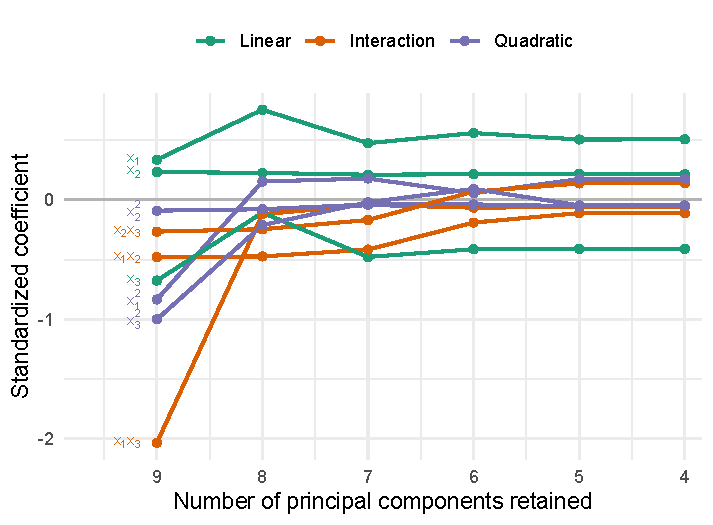
\includegraphics[width=\linewidth]{figures/acetylene_pcr.pdf}}
            \mode<article>{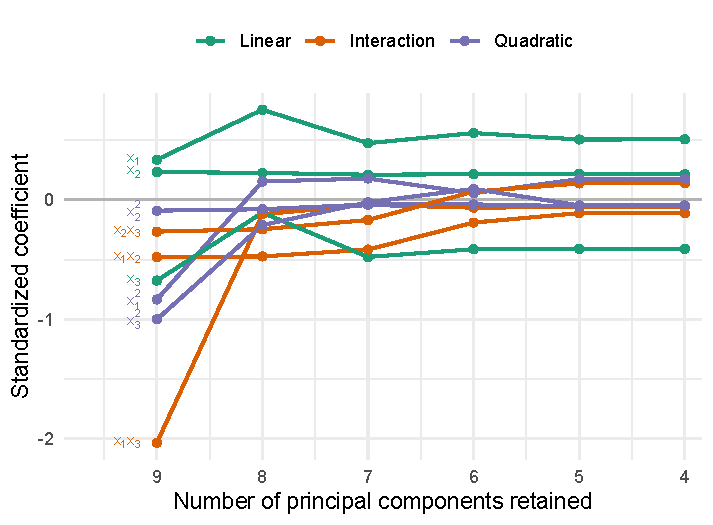
\includegraphics[width=0.8\linewidth]{figures/acetylene_pcr.pdf}}
        \end{column}
    \end{columns}
\end{frame}


\begin{frame}{Acetylene Data: Three Estimates Side by Side}
    \begin{columns}[T]
    \begin{column}{0.62\textwidth}
    \centering
        \footnotesize
        \begin{tabular}{lrrr}
            \toprule
            & LS & Ridge & PCR \\
            \midrule
            $x_1$ & 0.337 & 0.539 & 0.560 \\
            $x_2$ & 0.234 & 0.212 & 0.215 \\
            $x_3$ & $-0.676$ & $-0.374$ & $-0.413$ \\
            $x_1x_2$ & $-0.480$ & $-0.233$ & $-0.190$ \\
            $x_1x_3$ & $-2.034$ & $-0.068$ & $-0.065$ \\
            $x_2x_3$ & $-0.266$ & 0.012 & 0.069 \\
            $x_1^2$ & $-0.835$ & 0.125 & 0.056 \\
            $x_2^2$ & $-0.090$ & $-0.048$ & $-0.038$ \\
            $x_3^2$ & $-1.001$ & $-0.027$ & 0.092 \\
            \midrule
            $R^2$ & 0.9977 & 0.9944 & 0.9938 \\
            Largest VIF & 6563 & 4.18 & 8.27 \\
            \bottomrule
        \end{tabular}
    \end{column}
    \begin{column}{0.38\textwidth}
        \small
        Least squares (LS), ridge with $\theta=0.032$, PCR with $m=6$ components.
        \begin{itemize}
            \item Ridge and PCR agree closely with each other.
            \item Both differ sharply from least squares on the temperature and contact time terms.
            \item Both give up less than $0.004$ in $R^2$.
        \end{itemize}
    \end{column}
    \end{columns}
\end{frame}


\begin{frame}{Other Biased Estimators}
    \begin{itemize}
        \item \textbf{Lasso}: penalty $\theta\sum_j|b_j|$ instead of $\theta\sum_jb_j^2$. It shrinks and also sets some coefficients exactly to 0, so it selects regressors as well.
        \item \textbf{Elastic net}: a mix of the ridge and lasso penalties; useful when groups of correlated regressors should enter together.
        \item \textbf{Latent root regression} (Webster, Gunst and Mason, 1974): like PCR, but uses the eigenvectors of the correlation matrix of $y$ and the regressors together.
    \end{itemize}
    \svspace{0.5em}
    All trade a little bias for a large reduction in variance.
\end{frame}


\begin{frame}{Question: Why Accept a Worse Fit?}
    \begin{itemize}
        \item Ridge and PCR always have a larger $\SSRes$ than least squares on the same data. Why would we prefer them?
        \item Should the regressors be scaled before ridge regression? Does it matter?
    \end{itemize}
    % Answer:
    % - Least squares minimizes SSRes on this sample by construction; the goal is accurate coefficients and good predictions for new data, i.e. small mean squared error, not the smallest residuals here.
    % - With severe multicollinearity the least-squares coefficients are mostly noise along the small-eigenvalue directions; a small increase in SSRes buys a large drop in variance.
    % - Yes, scaling matters: the penalty theta * sum b_j^2 treats all coefficients alike, so the result depends on the units of each regressor. Unit-length (or standard-deviation) scaling puts all regressors on the same footing.
\end{frame}


\section{Summary}


\begin{frame}{Diagnostics at a Glance}
    \begin{center}
        \footnotesize
        \begin{tabular}{lll}
            \toprule
            Diagnostic & Warning level & What it shows \\
            \midrule
            Pairwise $r_{jl}$ & $|r_{jl}|$ near 1 & which pairs (misses larger groups) \\
            $\VIF_j=1/(1-R_j^2)$ & above 5 or 10 & which coefficients suffer \\
            $\kappa=\lambda_{\max}/\lambda_{\min}$ & 100--1000; above 1000 severe & overall severity \\
            $\kappa_j$ & above 1000 & how many dependencies \\
            Eigenvector $\bv_j$ & large loadings & which regressors are involved \\
            Proportions $\pi_{sj}$ & two or more above 0.5 & which coefficients each affects \\
            \bottomrule
        \end{tabular}
    \end{center}
\end{frame}


\begin{frame}{The Examples at a Glance}
    \begin{center}
        \footnotesize
        \begin{tabular}{llrrl}
            \toprule
            Data & Source & Largest VIF & $\kappa$ & Remedy shown \\
            \midrule
            Acetylene & sampling, model terms & 6563 & 43{,}381 & ridge, PCR \\
            Webster & constraint & 298 & 2196 & --- \\
            Gasoline (10 reg.) & population & 161 & 1820 & --- \\
            Hald cement & constraint & 283 & 1377 & drop $x_4$ \\
            Windmill & model terms & 38.5 & 152 & centering \\
            Delivery time & --- (mild) & 3.12 & 10.4 & none needed \\
            \bottomrule
        \end{tabular}
    \end{center}
\end{frame}


\begin{frame}{Key Takeaways}
    \begin{itemize}
        \item Multicollinearity is a near linear dependence among the regressors. Least squares stays unbiased, but its variances can be enormous.
        \item The data pin down combinations of correlated coefficients well and the individual coefficients poorly; prediction inside the data region is often fine.
        \item Pairwise correlations can miss a dependency; VIFs and the eigenvalues of $\bW'\bW$ do not.
        \item Eigenvectors and variance-decomposition proportions show which regressors are involved.
        \item Remedies: better data, a better parameterization, or a biased estimator such as ridge regression or PCR that trades a little bias for a large drop in variance.
    \end{itemize}
\end{frame}
